\section{Coherence}

The bandpass filter was designed to increase the $\kappa_r T_1$ product.
In Section \ref{sec:ch:results:characterization} we saw $\kappa_r$ values as fast as $1/19\,\text{ns}$.
It remains to see that the qubit $T_1$ was preserved.
We measured each qubit's $T_1$ over a range of frequencies, finding typical values between 10\,$\mu\text{s}$ and 12\,$\mu\text{s}$ over a range of qubit frequencies giving $\Delta > 800\,\text{MHz}$.
A full data set for qubit 2 is shown in Fig.\,\ref{Fig:ch:results:sec:coherence:swapSpectroscopyQ2}.
Without the filter, we expect a $T_1$ limit of $(\Delta/g)^2 / \kappa_r = 3.2\,\mu\text{s}$ at $\Delta=800\,\text{MHz}$.
As the measured $T_1$ values exceed that limit, we know that the filter successfully protected the qubit.
Of course, the qubit $T_1$ does not reach the upper limit allowed by the filter.
This was intentional, as we do not want the measurement circuit imposing additional decoherence of the qubit.
In other words, the qubit $T_1$ was dominated by loss channels other than the measurement circuit.

\begin{figure}
\begin{centering}
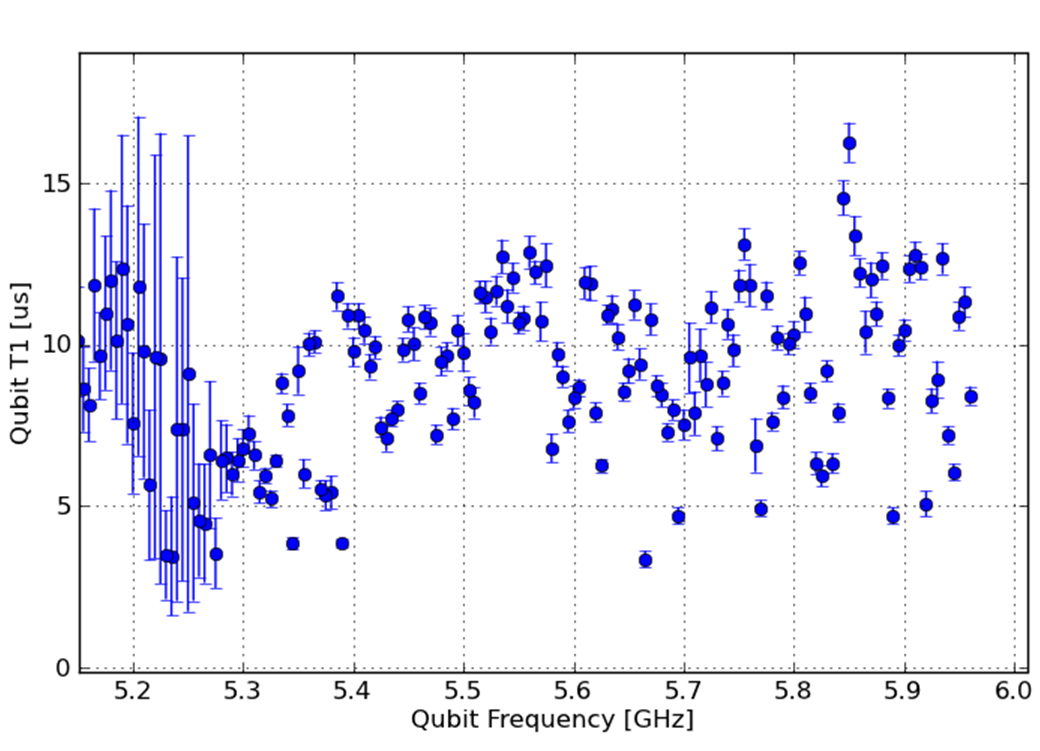
\includegraphics[width=\textwidth]{coherence.png}
\par\end{centering}
\caption{Energy decay time $T_1$ versus frequency for qubit $Q_2$.
With the measurement resonator frequency above the qubit, the lack of downward trend in $T_1$ with increasing qubit frequency indicates that the measurement circuit does not dominate the qubit damping.
The $T_1$ values are distributed around $10\,\mu\text{s}$, which is several times larger than the Purcell limit predicted in the absence of the filter.
The dip and wild variation in $T_1$ 5.2\,GHz come from coupling to a resonator bus which was not used in this experiment.}
\label{Fig:ch:results:sec:coherence:swapSpectroscopyQ2}
\end{figure}
